\documentclass[11pt,letterpaper]{article}
\usepackage[margin=0.85in]{geometry}
\usepackage[T1]{fontenc}
\usepackage{lmodern,microtype}
\usepackage{amsmath,amssymb,booktabs,tabularx,array}
\usepackage{graphicx,xcolor,caption,fancyhdr}
\usepackage[hidelinks]{hyperref}
\definecolor{navy}{HTML}{19354D}
\usepackage{titlesec}
\titleformat{\section}{\large\bfseries\color{navy}}{\thesection}{0.65em}{}
\titleformat{\subsection}{\normalsize\bfseries}{\thesubsection}{0.65em}{}
\titlespacing*{\section}{0pt}{13pt}{7pt}
\titlespacing*{\subsection}{0pt}{10pt}{5pt}
\captionsetup{font=small,labelfont=bf,skip=5pt}
\setlength{\parindent}{0pt}
\setlength{\parskip}{6pt}
\setlength{\intextsep}{6pt}
\setlength{\textfloatsep}{8pt}
\setlength{\floatsep}{8pt}
\setlength{\emergencystretch}{2em}
\renewcommand{\arraystretch}{1.2}
\pagestyle{fancy}
\fancyhf{}
\fancyhead[L]{\small Assignment 1: CartPole-v1}
\fancyhead[R]{\small Policy gradient}
\fancyfoot[C]{\small\thepage}
\setlength{\headheight}{14pt}
\graphicspath{{results/figures/}}
\newcommand{\E}{\mathbb{E}}
\newcommand{\norm}[1]{\left\lVert#1\right\rVert_\infty}
\newcommand{\argmin}{\operatorname*{arg\,min}}
\begin{document}
\begin{center}
{\LARGE\bfseries\color{navy} CartPole-v1}\\[5pt]
{\large Policy gradient with and without a baseline}
\end{center}

The primary basic-policy-gradient run achieved \textbf{500.00 $\pm$ 0.00} over 500 evaluation episodes. Adding a learned baseline reduced measured gradient variance at a fixed policy by \textbf{84.22\%}, but produced lower final evaluation scores in this training experiment. All three training seeds are reported below.

\section{Environment, notation, and objective}
The environment is \texttt{CartPole-v1}, run through Gymnasium 1.2.2, the maintained Gym successor. It uses the default reward of $+1$ per decision, including the terminal transition, and a 500-step limit. Actions push the cart left or right. The four observations are cart position, cart velocity, pole angle, and pole angular velocity. Physical failure occurs when the cart or pole crosses the allowed boundary.\footnote{Environment specification: \url{https://gymnasium.farama.org/environments/classic_control/cart_pole/}.}

\begin{table}[!ht]
\centering
\caption{Notation used in the algorithm.}
\begin{tabularx}{\linewidth}{@{}p{0.18\linewidth}X@{}}
\toprule
Symbol & Meaning\\
\midrule
$s_t$ & Four-component observation before decision $t$.\\
$a_t$ & Sampled action, 0 (left) or 1 (right).\\
$r_t$ & Reward received after action $a_t$; normally $+1$.\\
$T$ & Number of decisions in the current episode, at most 500.\\
$\theta$ & All weights and biases of the policy neural network.\\
$\pi_\theta(a\mid s)$ & Probability of selecting action $a$ in state $s$.\\
$\gamma$ & Discount factor, fixed at 0.95.\\
$G_t$ & Discounted reward still to be collected from decision $t$.\\
\bottomrule
\end{tabularx}
\end{table}

The discounted episodic objective and reward-to-go are
\begin{equation}
J(\theta)=\E_{\pi_\theta}\!\left[\sum_{t=0}^{T-1}\gamma^t r_t\right],
\qquad
G_t=\sum_{k=t}^{T-1}\gamma^{k-t}r_k.
\end{equation}
Here $\E_{\pi_\theta}$ means an average over episodes generated by the policy and environment. A larger $J$ is better. Compute $G_t$ backward: start with zero after the last reward and repeatedly apply $G_t=r_t+\gamma G_{t+1}$.

\textbf{Example.} Three rewards of $1$ give reward-to-go values $(2.8525,1.95,1)$ when $\gamma=0.95$. These are the learning targets. The \emph{plotted episode score} is instead the undiscounted sum $\sum_t r_t$, which is 3 in this example and at most 500 in CartPole.

All experiments used \textbf{CPU only and zero GPUs} on deepdish5. The code explicitly hides CUDA devices and uses one PyTorch/BLAS CPU thread.

\clearpage
\section{Implementation and comparison protocol}
\subsection{Basic REINFORCE}
The policy has four inputs, one hidden layer of 64 tanh units, and two output logits (unnormalized action scores). A categorical distribution converts the logits into action probabilities. Actions are sampled during both training and evaluation.

After collecting $B=32$ complete episodes, minimize the sampled loss
\begin{equation}
\mathcal L_{\rm actor}
=-\frac{1-\gamma}{B}\sum_{i=1}^{B}\sum_{t=0}^{T_i-1}
\gamma^t\log\pi_\theta(a_t^{(i)}\mid s_t^{(i)})
\bigl(G_t^{(i)}-b_t^{(i)}\bigr).
\label{eq:actor}
\end{equation}
The index $i$ identifies an episode, and $T_i$ its length. In the basic method, $b_t^{(i)}=0$. The gradient increases the probability of actions associated with larger discounted returns. Reward-to-go removes rewards occurring before an action, which cannot be affected by that action. The outer $\gamma^t$ is retained for the stated discounted episodic objective.

Adam uses the specified learning rate 0.01. The fixed factor $1-\gamma=0.05$ rescales the objective without changing its optimum. The gradient-norm cap is 10; it was never reached in any recorded run. Returns and advantages are \emph{not} normalized, so no implicit baseline is introduced in Part 1.

\subsection{Learned baseline for Part 2}
The baseline $b_\psi(s_t,t)$ predicts $G_t$, using a separate neural network with parameters $\psi$. It receives the four state components and elapsed time divided by 500, followed by 64 tanh units and one scalar output. Time is included because the remaining episode horizon can affect expected return.

Before each actor update, baseline predictions are computed and detached: the actor treats them as fixed numbers, and its loss does not update $\psi$. Afterward, the baseline receives five Adam updates at learning rate 0.01 to minimize the mean squared difference between predictions and full Monte Carlo targets $G_t$. There is no temporal-difference bootstrapping.

An action-independent baseline leaves the expected policy gradient unchanged because, conditional on the state and history,
\begin{equation}
\sum_a\pi_\theta(a\mid s)b\,\nabla_\theta\log\pi_\theta(a\mid s)
=b\,\nabla_\theta\sum_a\pi_\theta(a\mid s)=0.
\end{equation}
The symbol $\nabla_\theta$ denotes derivatives with respect to the policy parameters. Baseline fitting uses information from earlier batches before the current actions are collected, avoiding dependence of the current baseline on its sampled action.

\subsection{Training and evaluation protocol}
Each method trains for 8,000 episodes (250 updates) using seeds 1668, 1669 and 1670. Seed 1668 was fixed as the primary run before full training. A 1,024-episode basic-method pilot checked functionality at learning rate 0.01 and is archived separately. The full runs restart from their seeds. Actor initialization, reset-seed schedule, learning rate and episode budget are matched across methods.

Every final checkpoint is evaluated over 500 fresh episodes, with reset seeds 9000000--9000499 shared across methods. Training does not use these resets. No checkpoint is selected using evaluation performance. Evaluation keeps stochastic actions and never updates weights. Standard deviations reported below use the population formula over the 500 episode scores.

\clearpage
\section{Part 1(a): basic policy gradient results}
For the primary seed, the final policy achieved 500 in every evaluation episode: mean \textbf{500.000}, standard deviation \textbf{0.000}. All 500 episodes reached the time limit. This is strong evidence for that particular model on the evaluated reset distribution, not proof that every training seed converges.

\begin{figure}[!ht]
\centering
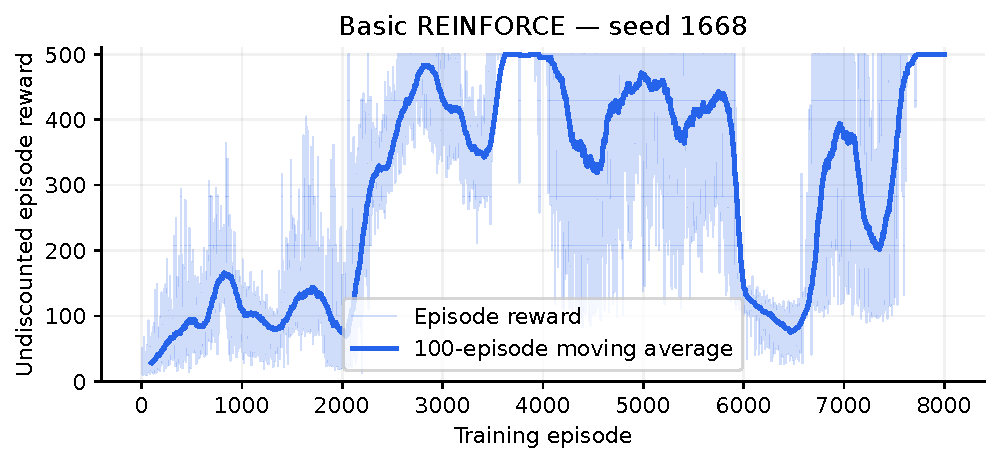
\includegraphics[width=0.93\linewidth]{no_baseline_training.pdf}
\caption{Basic REINFORCE: raw episode rewards and the trailing 100-episode moving average, starting at episode 100. Training seed 1668.}
\end{figure}

\begin{figure}[!ht]
\centering
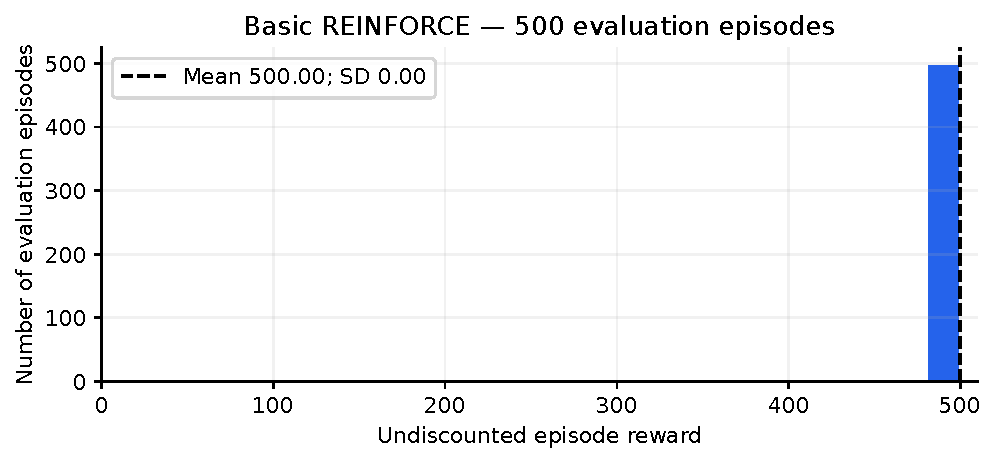
\includegraphics[width=0.93\linewidth]{no_baseline_evaluation_histogram.pdf}
\caption{Basic REINFORCE: histogram of 500 fresh evaluation scores. The mass lies in the final bin because all scores are 500.}
\end{figure}

A uniform random policy scored $22.782\pm12.058$ over 500 episodes. The untrained primary neural policy scored $20.926\pm11.467$. These references support a substantial learned improvement rather than good performance from initialization alone.

\clearpage
\section{Part 2: results with a learned baseline}
For the primary seed, the baseline model scored \textbf{260.308 $\pm$ 57.013}. Four of its 500 evaluation episodes reached the time limit; 496 ended through physical failure. It improved substantially over the random and untrained references but underperformed the primary basic-method model.

\begin{figure}[!ht]
\centering
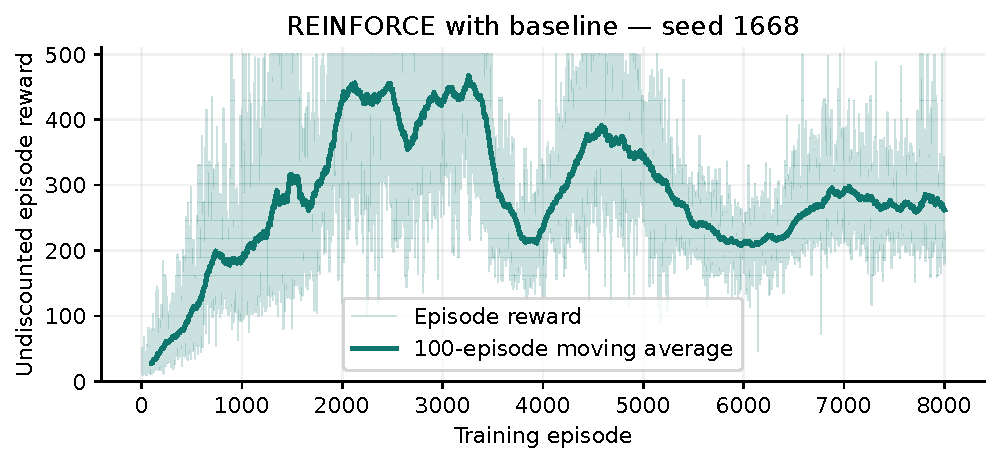
\includegraphics[width=0.93\linewidth]{baseline_training.pdf}
\caption{REINFORCE with learned baseline: episode rewards and the trailing 100-episode moving average. Training seed 1668.}
\end{figure}

\begin{figure}[!ht]
\centering
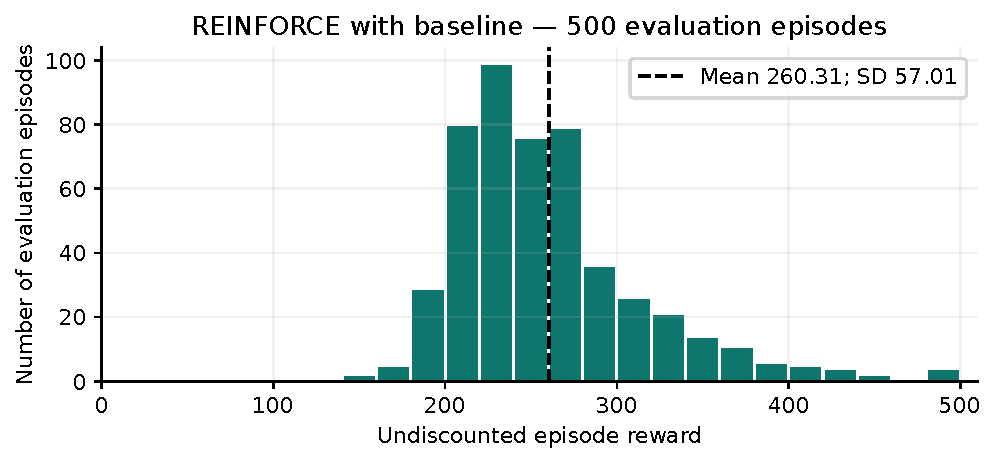
\includegraphics[width=0.93\linewidth]{baseline_evaluation_histogram.pdf}
\caption{Learned-baseline policy: histogram of 500 fresh evaluation scores, with mean 260.308 and population standard deviation 57.013.}
\end{figure}

The baseline method receives exactly the same number of environment episodes as the basic method, but performs additional computation to fit its value predictor. Lower estimator variance alone does not guarantee a better final policy under a fixed training budget.

\clearpage
\section{Across-seed results and the variance experiment}
\begin{table}[!ht]
\centering
\caption{Every final model, each evaluated on 500 fresh episodes. Within-row SD describes variation among episodes for one fixed model.}
\begin{tabular}{lrrrr}
\toprule
Method & Training seed & Mean score & SD & Fraction at 500\\
\midrule
No baseline & 1668 & 500.000 & 0.000 & 1.000\\
No baseline & 1669 & 271.824 & 28.856 & 0.000\\
No baseline & 1670 & 483.886 & 65.298 & 0.928\\
\midrule
Learned baseline & 1668 & 260.308 & 57.013 & 0.008\\
Learned baseline & 1669 & 360.516 & 79.141 & 0.100\\
Learned baseline & 1670 & 349.940 & 76.321 & 0.092\\
\bottomrule
\end{tabular}
\end{table}

The mean of the three seed-specific evaluation means was 418.570 without the baseline and 323.588 with it. The corresponding sample SDs across seed means were 127.341 and 55.057. These are different quantities from within-model episode SD. Three seeds show sensitivity to initialization and sampling but are insufficient for a broad statistical claim. The baseline was better for seed 1669, but worse for the other two seeds and lower on average.

\subsection{Does the baseline actually reduce gradient variance?}
Comparing training reward variance cannot isolate this question because the policies change. Instead, freeze one initial policy. Fit a baseline on 512 independent episodes, then calculate both gradient estimators on the \emph{same} 512 different trajectories. For each policy parameter, calculate its sample gradient variance, and sum these variances. This sum is the trace of the gradient covariance matrix.

\begin{table}[!ht]
\centering
\caption{Paired gradient-variance measurement at one frozen policy.}
\begin{tabular}{lr}
\toprule
Estimator & Sum of parameter variances\\
\midrule
No baseline & 5.338262\\
Learned baseline & 0.842421\\
\bottomrule
\end{tabular}
\end{table}

The measured reduction was $1-0.842421/5.338262=84.22\%$. The distance between the two empirical mean gradients was 0.0474, compared with a root-sum-squared standard error of 0.1176 for their paired difference. Finite-sample mean agreement is consistent with the analytic baseline-invariance property; it is not itself a proof. The experiment demonstrates variance reduction at this frozen initial policy, not at every later training policy.

\subsection{Discounted objective versus episode score}
With reward $+1$ each step, a length-$T$ episode has discounted return
\begin{equation}
\frac{1-0.95^T}{1-0.95},
\end{equation}
which approaches 20. The primary baseline policy's average discounted evaluation return was 19.999743, while the basic model's was approximately 20.000000, despite their large difference in undiscounted scores. Discounting therefore makes extra survival late in an episode a weak objective signal. This observation explains a limitation of the required objective, without establishing the cause of the baseline method's lower final score.

\clearpage
\section{Edge cases and correctness validation}
\subsection{Predictable calculations and policy updates}
\textbf{Discounting.} For rewards $(1,1,1)$, backward calculation produces $(2.8525,1.95,1)$; implementation values match to floating-point precision. Setting $\gamma=0$ produces the immediate rewards exactly.

\textbf{Exact policy-gradient example.} In a two-step toy environment, let both actions be sampled from a Bernoulli probability $p=\operatorname{sigmoid}(\theta)$ and let each reward equal its binary action. The exact objective is $(1+\gamma)p$, with derivative $(1+\gamma)p(1-p)$. Enumerating all four possible action sequences gave gradient 0.471188756 with or without a constant baseline; the analytic derivative was 0.471188748. This checks the return-to-go estimator, outer discount factor, and baseline invariance.

\textbf{Gradient direction.} A positive-reward update for one selected action increased its probability from 0.500000 to 0.502500. A wrong sign in the actor loss would reverse this direction.

\subsection{Environment end conditions and reproducibility}
Fixed reset seeds and a fixed ten-action sequence reproduced the same states exactly. Deliberately placing the cart beyond the position boundary and the pole beyond its angle boundary separately produced physical termination. Each terminating step still delivered reward $+1$.

A one-step time-limit experiment produced truncation without physical termination. Training and evaluation stop on either flag. Because the objective is a complete finite episode, returns end at that boundary and do not bootstrap from a later state. The environment is reset before another episode, and return accumulation never crosses episode boundaries.

\subsection{Inspecting ten actual decisions}
The file \path{validation/first_ten_steps.csv} records the four state components, probability of moving right, sampled action, reward and end flags. The primary basic-policy-gradient checkpoint was used, with reset seed 9100000 and action-sampling seed 123456. The first decisions illustrate the distinction between action probability and action selection:

\begin{table}[!ht]
\small
\centering
\caption{Excerpt of the saved trace. Angles are in radians.}
\begin{tabular}{rrrrrrr}
\toprule
$t$ & Position & Velocity & Angle & Angular velocity & $P(\text{right})$ & Action\\
\midrule
0 & 0.01276 & -0.01188 & -0.04659 & -0.03077 & 0.1019 & Left\\
1 & 0.01252 & -0.20630 & -0.04721 & 0.24686 & 0.8335 & Right\\
2 & 0.00840 & -0.01054 & -0.04227 & -0.06033 & 0.0700 & Left\\
3 & 0.00818 & -0.20503 & -0.04348 & 0.21872 & 0.7711 & Left\\
\bottomrule
\end{tabular}
\end{table}

All four rewards were 1. At decision 3, the less likely left action was sampled even though the probability of right was 0.7711. This is valid stochastic behavior, not a mismatch between the network and environment. The full trace permits further manual inspection rather than relying only on an aggregate learning curve.

\clearpage
\section{Reproduction, limitations, and additional experiments}
The training code, final and initial model checkpoints, configurations, evaluation rewards and logs are saved in \path{mlds_assignment1_cartpole}. On deepdish5, the environment is already installed. Run:
\begin{verbatim}
cd ~/mlds_assignment1_cartpole
source ~/mlds_assignment1_cartpole_env/bin/activate
python cartpole.py suite --episodes 8000 --lr 0.01
python validate.py
\end{verbatim}
This regenerates and overwrites the six run folders; preserve the original results if desired. To inspect saved results without training, open \path{cartpole_plots.ipynb} and run all cells. The notebook needs only NumPy, Matplotlib and Jupyter. It generates the required reward curves, 100-episode moving averages and 500-episode histograms, as well as additional comparison figures.

Per-run \path{config.json} files record the actual software and settings: Python 3.12, PyTorch 2.14.0+cu130, NumPy 2.5.3 and Gymnasium 1.2.2. Although the installed PyTorch supports CUDA, all experiments used CPU. Full validation evidence is in \path{validation/validation.json}, with paired sample gradients in \path{validation/gradient_variance.npz}.

\subsection{Limits of the evidence}
The primary basic-policy-gradient model reached the maximum in all 500 trials, but this did not occur for every seed. Likewise, the baseline's variance reduction at a frozen initial policy did not imply better final performance. The learned value approximation, finite data and evolving policy all merit further investigation. The experiments do not establish which factor caused the difference, and no evaluation-based hyperparameter or checkpoint selection was used to improve the reported results.

\subsection{With an additional three months}
First, run more training seeds and tune learning rate, episode batch size and critic-fitting frequency using \emph{separate validation seeds}. Reserve another reset-seed set for final evaluation. This would distinguish reproducible improvements from favorable individual runs.

Second, repeat paired variance measurements at early, middle and late policy checkpoints. Compare a constant baseline, the current state/time baseline, and different critic capacities. Measure value-prediction error alongside gradient variance and average gradient direction. These experiments would test whether inaccurate or outdated predictions limit the baseline during training.

Finally, study robustness under perturbed reset states, pole lengths and cart/pole masses. Evaluate stochastic and greedy policies separately, and measure the impact of truncation and the required discount factor. Any alternative discounting should be an additional sensitivity experiment, with the assignment's $\gamma=0.95$ results retained as the main comparison.
\end{document}
